%!TEX program = pdflatex
\documentclass[aspectratio=169,10pt]{beamer}

\usetheme{Madrid}
\usecolortheme{seahorse}

\setbeamertemplate{footline}[frame number]

% Packages
\usepackage{amsmath}
\usepackage{amssymb}
\usepackage{amsfonts}
\usepackage{graphicx}
\usepackage{listings}
\usepackage{xcolor}
\usepackage{subcaption}
\usepackage{multirow}
\usepackage{array}

% Graphics path
\graphicspath{{figures/}}

% Code listing style
\lstset{
    basicstyle=\ttfamily\scriptsize,
    keywordstyle=\color{blue},
    commentstyle=\color{green!50!black}\itshape,
    stringstyle=\color{red},
    breaklines=true,
    numbers=left,
    numberstyle=\tiny\color{gray},
    frame=single,
    breakatwhitespace=false,
    tabsize=2
}

% Title page
\title[Chapter 4d: Fixed Point Theorems in Banach Algebra and Lattices]{
    Fixed Point Theorems in Banach Algebra\\[0.3cm]
    and\\[0.3cm]
    Lattice-Theoretic Fixed Point Theorems
}
\subtitle{Iterative Methods and Approximation (Sections 5.8--5.9)}

\author{Based on Pathak: An Introduction to Nonlinear Analysis and Fixed Point Theory}
\date{\today}

\begin{document}

\frame{\titlepage}

% Outline
\begin{frame}
    \frametitle{Overview}
    \tableofcontents
\end{frame}

% Section 1: Contraction and Lipschitz mappings
\section{Contraction Mappings and Lipschitzian Operators}

\begin{frame}[fragile]{Fundamental Concepts}
    \begin{definition}[Nonlinear Contraction - Definition 5.92]
        A mapping $T: X \to X$ on a Banach space $X$ is a \textbf{nonlinear contraction} if:
        \[
            \|Tx - Ty\| \leq \phi(\|x - y\|), \quad \forall x, y \in X,
        \]
        where $\phi: \mathbb{R}^+ \to \mathbb{R}^+$ is continuous with $\phi(r) < r$ for all $r > 0$.
    \end{definition}

    \begin{definition}[$\mathcal{D}$-Lipschitzian Mappings - Definition 5.93]
        A mapping $T: X \to X$ is \textbf{$\mathcal{D}$-Lipschitzian} (Dhage, 2003) if:
        \[
            \|Tx - Ty\| \leq \phi(\|x - y\|), \quad \forall x, y \in X,
        \]
        where $\phi: \mathbb{R}^+ \to \mathbb{R}^+$ is continuous and nondecreasing with $\phi(0) = 0$.
    \end{definition}

    \textbf{Key difference:} Nonlinear contractions require $\phi(r) < r$, while $\mathcal{D}$-Lipschitzian
    mappings only require $\phi(0) = 0$.
\end{frame}

\begin{frame}{Classification of Operators}
    \begin{itemize}
        \item \textbf{Compact Operator}: $T(X)$ is a compact subset of $X$
        \begin{itemize}
            \item Every bounded sequence in $T(X)$ has a convergent subsequence
        \end{itemize}
        \vspace{0.3cm}

        \item \textbf{Totally Bounded Operator}: For any bounded $S \subseteq X$, $T(S)$ is totally bounded
        \begin{itemize}
            \item Can be covered by finitely many $\varepsilon$-balls for any $\varepsilon > 0$
        \end{itemize}
        \vspace{0.3cm}

        \item \textbf{Completely Continuous Operator}: Both continuous and totally bounded
        \begin{itemize}
            \item Every compact operator is completely continuous
            \item But converse may not hold
        \end{itemize}
    \end{itemize}

    \vspace{0.5cm}
    \textbf{Relationship:} Compact $\Rightarrow$ Totally bounded $\Rightarrow$ Completely continuous
\end{frame}

\begin{frame}{Illustration of Operator Types}
    \begin{figure}[h]
        \centering
        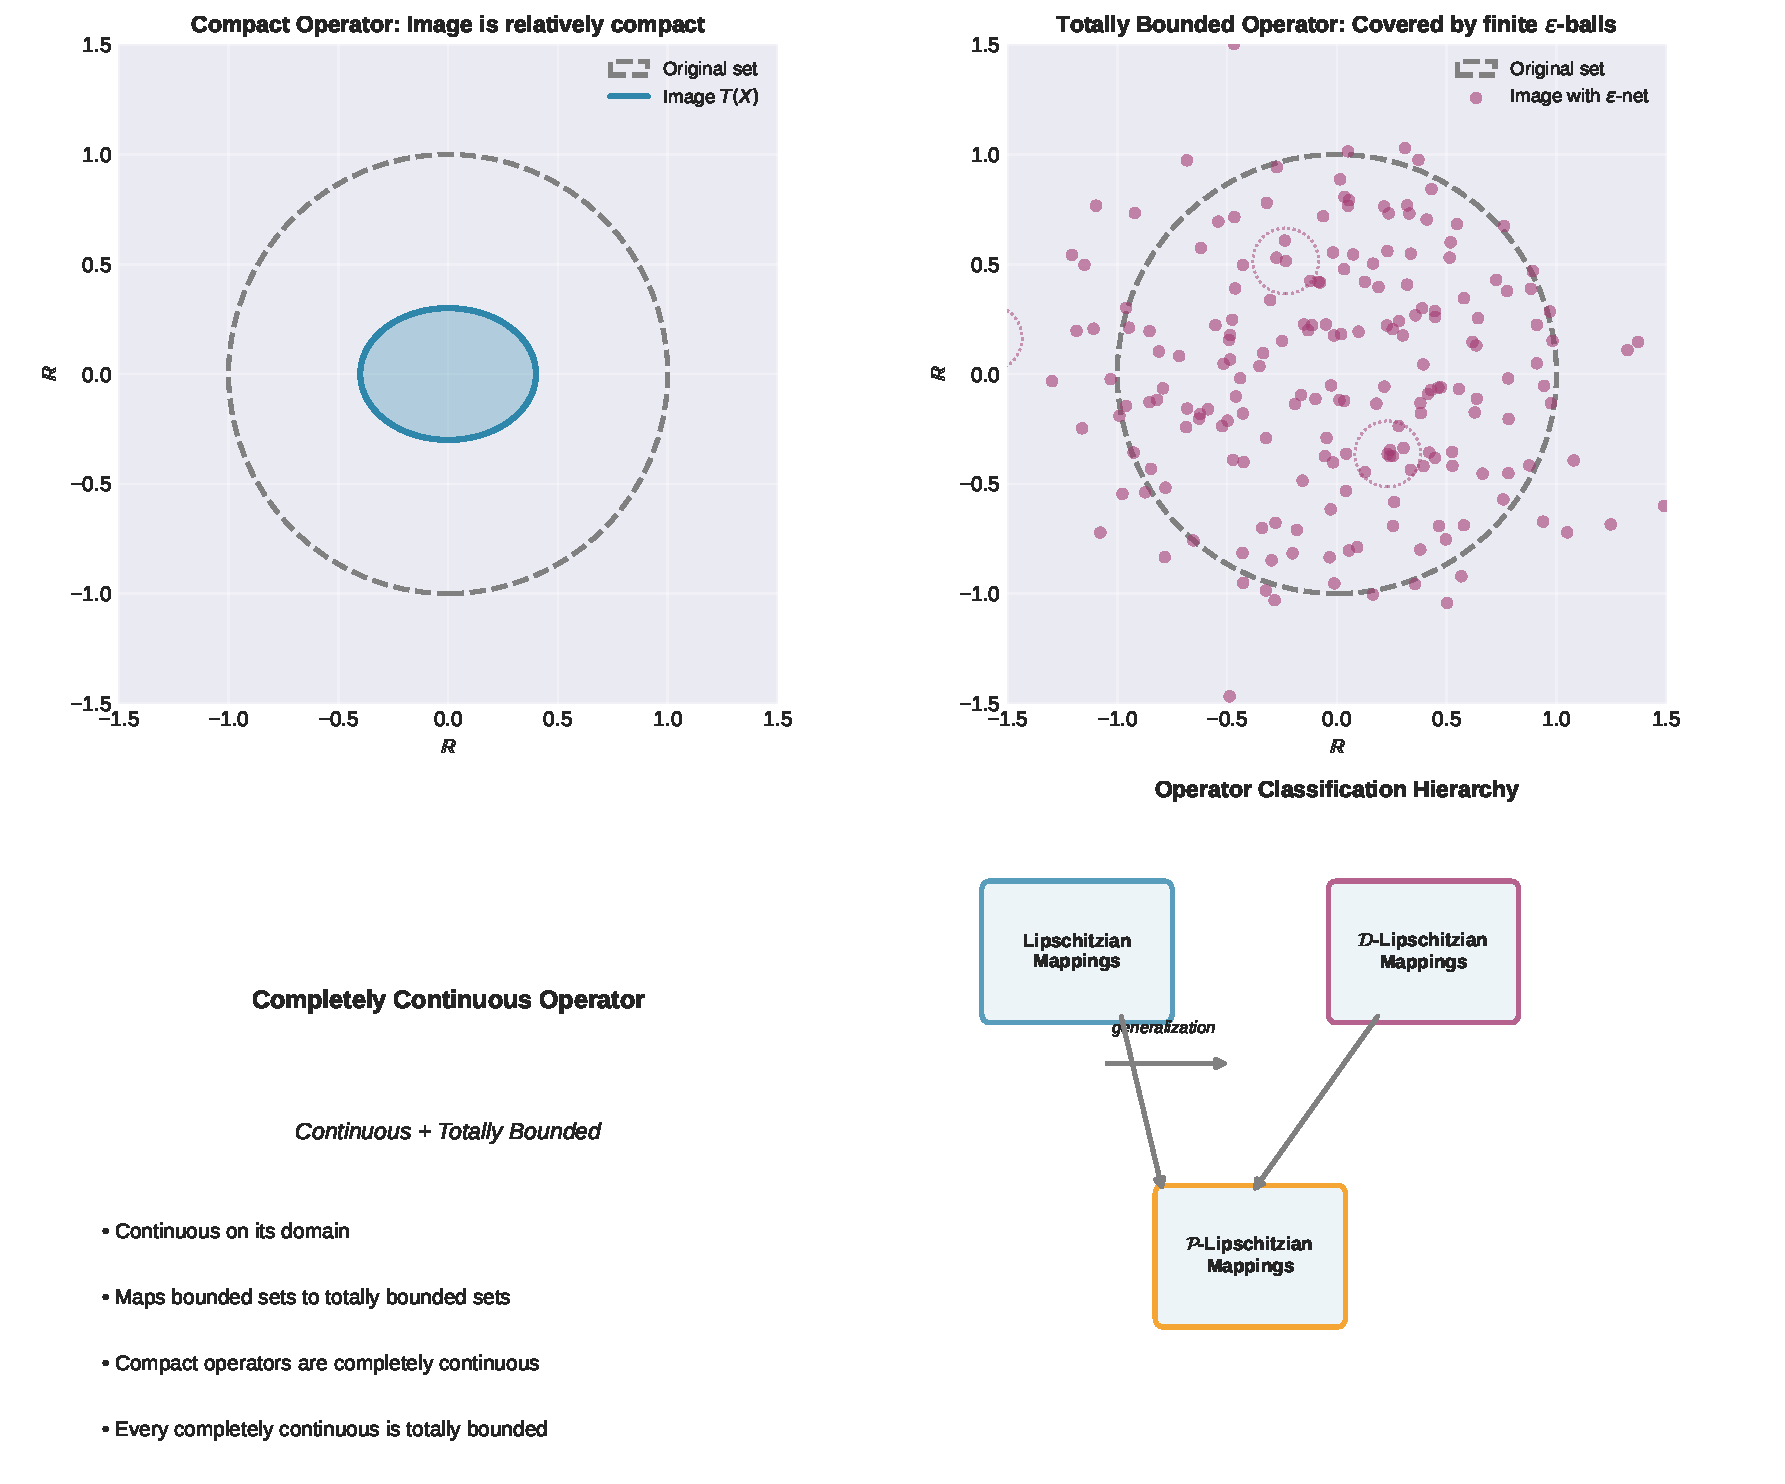
\includegraphics[width=\textwidth]{fig_operator_types.pdf}
    \end{figure}
\end{frame}

% Section 2: Fixed Point Theorems in Banach Algebra
\section{Fixed Point Theorems in Banach Algebra}

\begin{frame}[allowframebreaks]{Krasnoselski Fixed Point Theorem}
    \begin{theorem}[Krasnoselski - Theorem 5.176]
        Let $S$ be a closed, convex, and bounded subset of a Banach algebra $X$.
        Let $A, B: S \to X$ be two operators such that:
        \begin{enumerate}
            \item[(a)] $A$ is a contraction;
            \item[(b)] $B$ is completely continuous; and
            \item[(c)] $Ax + By \in S$, $\forall x, y \in S$.
        \end{enumerate}
        Then the operator equation
        \[
            Ax + Bx = x
        \]
        has a solution in $S$.
    \end{theorem}

    \textbf{Significance:}
    \begin{itemize}
        \item Decomposes the fixed point problem into a contraction and a compact perturbation
        \item Enables treatment of more complex operator equations
        \item Foundation for many applications in differential and integral equations
    \end{itemize}
\end{frame}

\begin{frame}{Burton's Modification}
    \begin{theorem}[Burton - Theorem 5.177]
        Let $S$ be a closed, convex, and bounded subset of a Banach algebra $X$.
        Let $A: X \to X$ and $B: S \to X$ be two operators such that:
        \begin{enumerate}
            \item[(a)] $A$ is a contraction;
            \item[(b)] [Weaker condition] $B: S \to X$ satisfies a mild boundedness condition; and
            \item[(c)] [Weaker covering] A milder covering condition replacing (c) from Krasnoselski.
        \end{enumerate}
        Then $Ax + Bx = x$ has a solution in $S$.
    \end{theorem}

    \textbf{Key Innovation:}
    \begin{itemize}
        \item Burton weakened Krasnoselski's stringent hypothesis (c)
        \item $B$ need not be completely continuous---only bounded
        \item More applicable to practical problems
    \end{itemize}
\end{frame}

\begin{frame}[fragile]{$\mathcal{P}$-Lipschitzian Fixed Point Theorem}
    \begin{theorem}[Theorem 5.184]
        Let $S$ be a closed, convex, and bounded subset of a Banach space $X$.
        Let $A: X \to X$ and $B: S \to X$ be two operators such that:
        \begin{enumerate}
            \item[(a)] $A$ is a $\mathcal{P}$-Lipschitzian contraction;
            \item[(b)] $B$ is completely continuous; and
            \item[(c)] $\|x\| \leq \|Ax + By\|$, $\forall x \in X, y \in S$.
        \end{enumerate}

        If $M\phi(r) + \phi_C(r) < r$ for $r > 0$, where $M = \|B(S)\|$,
        then $Ax + Bx = x$ has a solution, whenever $M\phi(r) < r$.
    \end{theorem}

    \begin{lstlisting}[language=Python, caption=Verification of $\mathcal{P}$-Lipschitzian condition]
# Example: Checking contractiveness condition
import numpy as np

def phi(r):
    """Example $\mathcal{P}$-Lipschitzian function"""
    return 0.5 * r  # Linear case

r_values = np.linspace(0.1, 10, 100)
M = 2.0  # Bound on operator B

# Check if M*phi(r) < r (contractiveness condition)
contractiveness = M * np.array([phi(r) for r in r_values]) < r_values

# Region where contractiveness holds
valid_r = r_values[contractiveness]
print(f"Contractiveness holds for r > {r_values[~contractiveness][-1]:.2f}")
    \end{lstlisting}
\end{frame}

\begin{frame}[fragile]{$\mathcal{D}$-Lipschitzian Fixed Point Theorem}
    \begin{theorem}[Theorem 5.185]
        Let $S$ be a closed, convex, and bounded subset of a Banach algebra $X$.
        Let $A: X \to X$ and $B: S \to X$ be two operators such that:
        \begin{enumerate}
            \item[(a)] $A$ is $\mathcal{D}$-Lipschitzian;
            \item[(b)] $B$ is completely continuous; and
            \item[(c)] $x = Ax By \Rightarrow x \in S$, $\forall y \in S$.
        \end{enumerate}

        Then the operator equation $AxBy = x$ has a solution whenever
        $M\phi(r) < r, r > 0$, where $M = \|B(S)\|$.
    \end{theorem}

    \begin{definition}[Sufficient Condition - Proposition 5.14]
        If $S = \{y \in X : \|y\| \leq r\}$ and
        \[
            \|x\| \leq \left\| \left( I - C \right) x \right\|, \quad \forall x \in X,
        \]
        then hypothesis (c) is satisfied in Theorem 5.177.
    \end{definition}
\end{frame}

\begin{frame}{Convergence and Iteration}
    \begin{figure}[h]
        \centering
        
\includegraphics[width=\textwidth]{fig_iteration_convergence.pdf}
    \end{figure}

    \textbf{Convergence Comparison:}
    \begin{itemize}
        \item \textbf{Banach Contraction:} Exponential convergence, guaranteed for $k < 1$
        \item \textbf{Mann Iteration:} Slower (sublinear) for nonexpansive mappings
        \item \textbf{Krasnoselski Method:} Combines benefits of both approaches
    \end{itemize}
\end{frame}

\begin{frame}[fragile]{Numerical Example: Computing Fixed Points}
    \begin{lstlisting}[language=Python, caption=Fixed point iteration for Krasnoselski operator]
import numpy as np
from numpy.linalg import norm

def contraction_A(x, k=0.5):
    """Contraction operator: A(x) = k*x"""
    return k * x

def compact_B(x, epsilon=0.1):
    """Compact perturbation: B(x) = epsilon*sin(x)"""
    return epsilon * np.sin(x)

def krasnoselski_iterate(x, alpha=0.5):
    """Krasnoselski iteration: x_{n+1} = A(x_n) + B(x_n)"""
    return contraction_A(x) + compact_B(x)

# Fixed point iteration
x = np.array([1.0, 2.0, 3.0])
errors = []
for n in range(20):
    x_old = x.copy()
    x = krasnoselski_iterate(x)
    error = norm(x - x_old)
    errors.append(error)
    if n < 5 or n >= 18:
        print(f"Iter {n:2d}: ||x_new - x_old|| = {error:.6e}")
    elif n == 5:
        print("...")

print(f"\nConverged: {error < 1e-10}")
    \end{lstlisting}
\end{frame}

\begin{frame}{Relationship Between Operator Types}
    \begin{figure}[h]
        \centering
        
\includegraphics[width=\textwidth]{fig_contraction_mapping.pdf}
    \end{figure}

    \textbf{Key Insights:}
    \begin{itemize}
        \item Contraction mapping: Every iteration brings points closer to fixed point
        \item Fixed point is unique and guaranteed to exist (Banach Contraction Principle)
        \item Iteration sequence $\{x_n\}$ converges exponentially fast
    \end{itemize}
\end{frame}

% Section 3: Lattice-Theoretic Fixed Points
\section{Lattice-Theoretic Fixed Point Theorems}

\begin{frame}{Ordered Banach Spaces and Lattices}
    \begin{definition}[Partially Ordered Set]
        A set $X$ with a binary relation $\leq$ is \textbf{partially ordered} if for all $x,y,z \in X$:
        \begin{enumerate}
            \item Reflexivity: $x \leq x$
            \item Antisymmetry: $x \leq y$ and $y \leq x$ $\Rightarrow$ $x = y$
            \item Transitivity: $x \leq y$ and $y \leq z$ $\Rightarrow$ $x \leq z$
        \end{enumerate}
    \end{definition}

    \begin{definition}[Complete Lattice]
        A poset $L$ is a \textbf{complete lattice} if every subset has both a least upper bound (supremum)
        and a greatest lower bound (infimum).
    \end{definition}

    \textbf{Examples:}
    \begin{itemize}
        \item Power set $2^X$ (all subsets of $X$)
        \item Intervals in $\mathbb{R}$: $[a,b]$ with usual ordering
        \item Banach lattices: Normed vector lattices with order-continuous norm
    \end{itemize}
\end{frame}

\begin{frame}[allowframebreaks]{Knaster-Tarski Fixed Point Theorem}
    \begin{theorem}[Knaster-Tarski (1927)]
        Let $f: L \to L$ be a monotone increasing function on a complete lattice $L$.
        Then:
        \begin{enumerate}
            \item The set of fixed points $\text{Fix}(f) = \{x \in L : f(x) = x\}$ is non-empty.
            \item The set of fixed points itself forms a complete lattice.
            \item The function $f$ has a least fixed point and a greatest fixed point.
        \end{enumerate}
    \end{theorem}

    \textbf{Key Advantage:}
    \begin{itemize}
        \item Does \textbf{not} require continuity of $f$
        \item Applies to discrete structures and infinite-dimensional spaces
        \item Guarantees existence without constructive iteration
    \end{itemize}

    \framebreak

    \textbf{Proof Strategy:}
    \begin{itemize}
        \item Consider the set of prefixed points: $A = \{x \in L : x \leq f(x)\}$
        \item If $x \leq f(x)$, then $f(x) \leq f(f(x))$ (by monotonicity)
        \item The supremum $x^* = \sup A$ satisfies $f(x^*) = x^*$
        \item This $x^*$ is the least fixed point
        \item Similarly, there exists a greatest fixed point
    \end{itemize}
\end{frame}

\begin{frame}{Monotone Functions and Fixed Points}
    \begin{figure}[h]
        \centering
        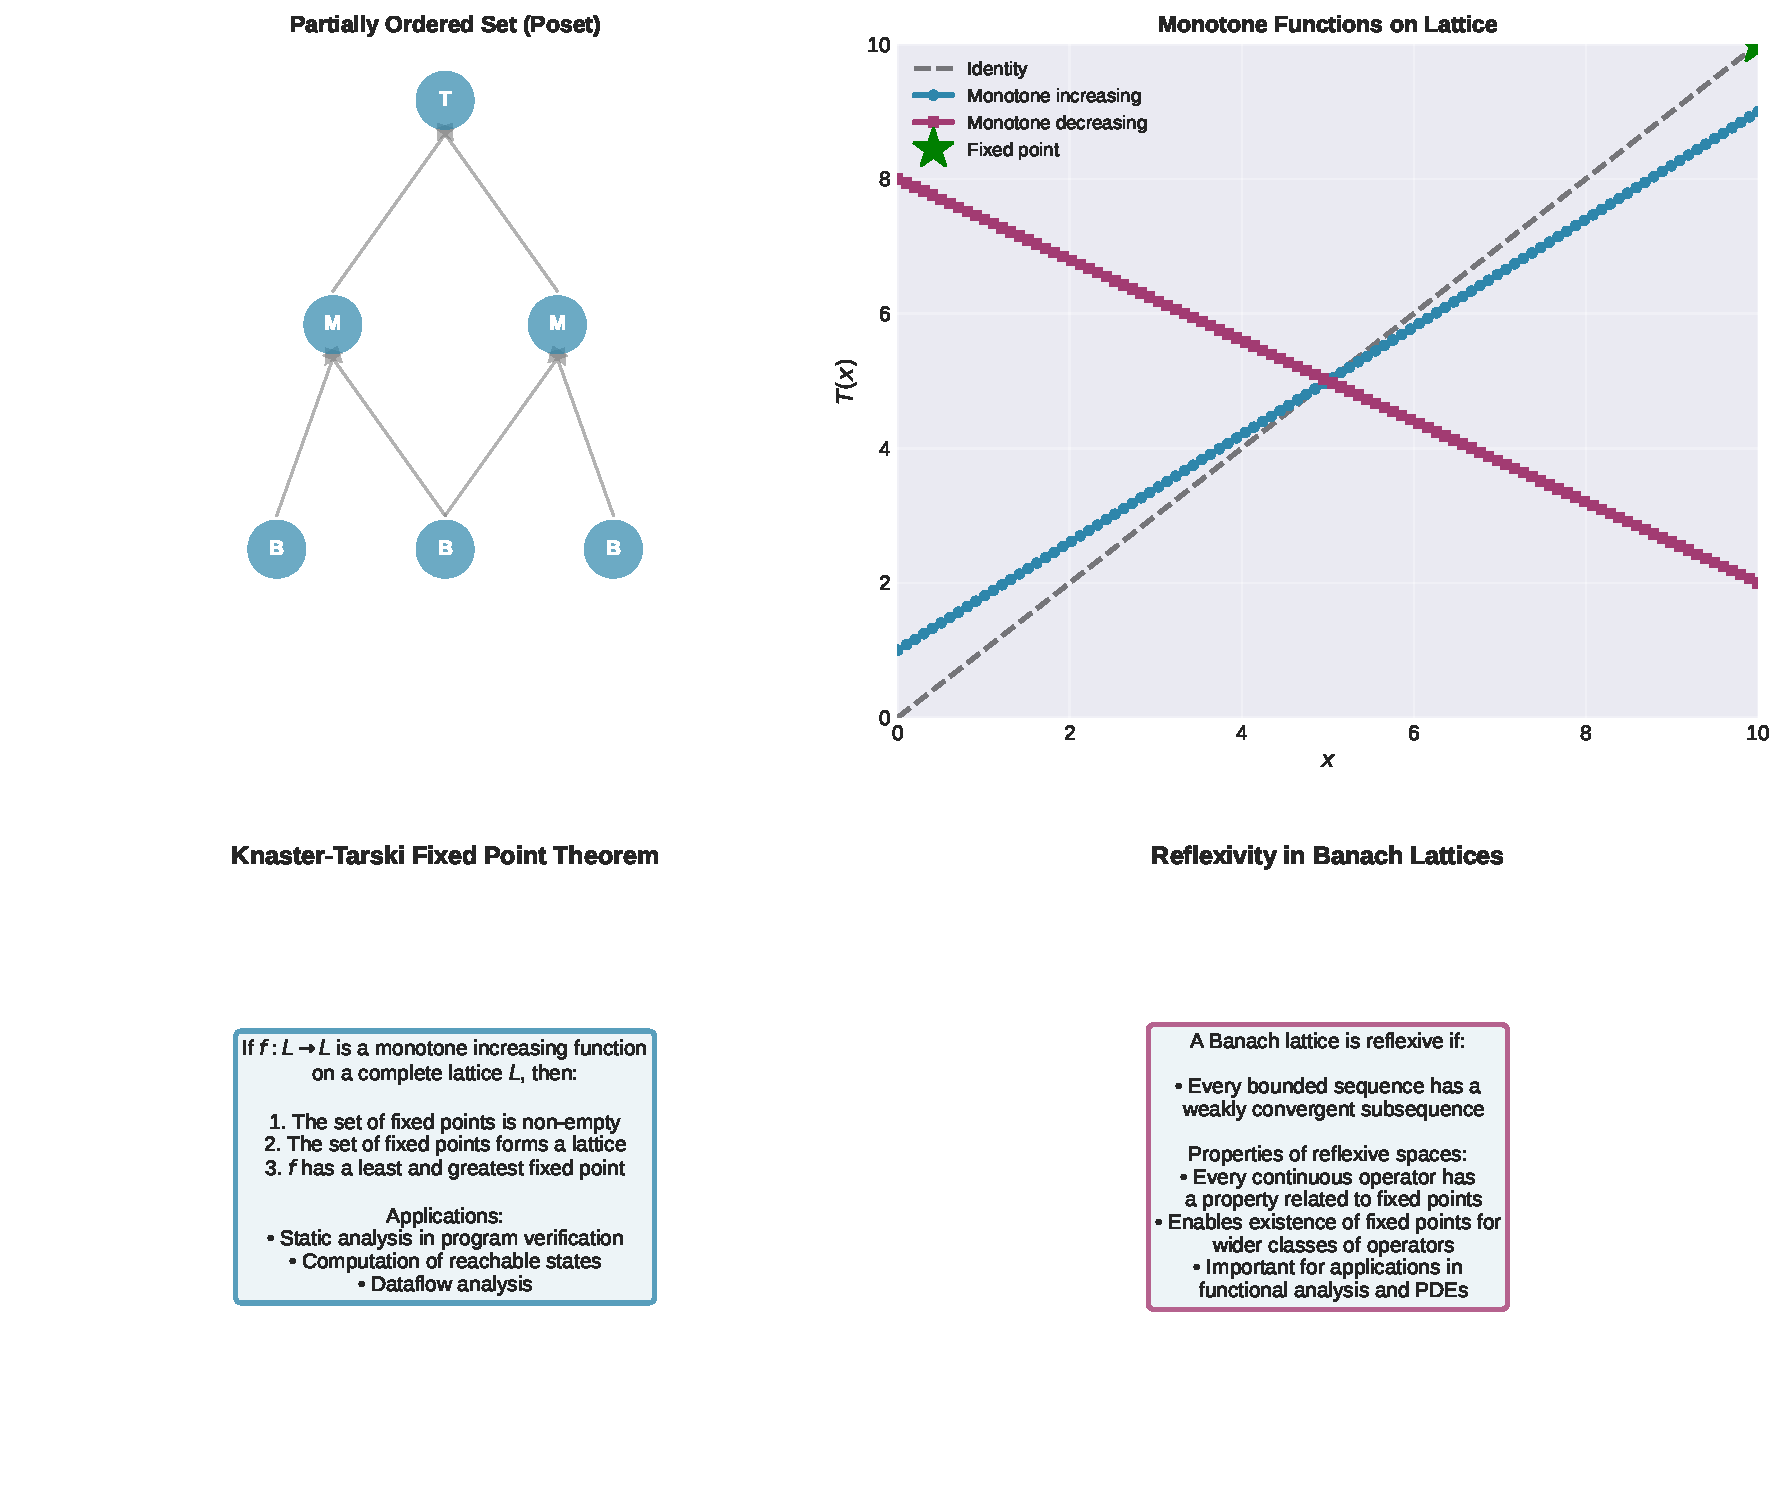
\includegraphics[width=\textwidth]{fig_lattice_fixed_points.pdf}
    \end{figure}

    \textbf{Important observations:}
    \begin{itemize}
        \item Monotone increasing functions preserve order: $x \leq y \Rightarrow f(x) \leq f(y)$
        \item Fixed points form a lattice structure themselves
        \item Applicable to program verification and static analysis
    \end{itemize}
\end{frame}

\begin{frame}{Applications of Lattice Fixed Points}
    \textbf{Computer Science Applications:}
    \begin{itemize}
        \item \textbf{Program Verification:} Computing fixed points of program transformations
        \item \textbf{Dataflow Analysis:} Finding reachable states in control flow graphs
        \item \textbf{Abstract Interpretation:} Analyzing program properties using abstract domains
    \end{itemize}

    \vspace{0.5cm}
    \textbf{Mathematical Applications:}
    \begin{itemize}
        \item Fixed points of increasing operators in Banach lattices
        \item Existence of solutions to functional inequalities
        \item Properties of measure-preserving transformations
    \end{itemize}

    \vspace{0.5cm}
    \textbf{Example (Reachability in graphs):}
    \begin{itemize}
        \item Let $L = 2^V$ be the powerset of vertices
        \item $f(S) = S \cup \{v : \exists u \in S, (u,v) \in E\}$
        \item The least fixed point is the set of reachable vertices
    \end{itemize}
\end{frame}

\begin{frame}{Reflexivity and Cascading Nonexpansive Maps}
    \begin{theorem}[Section 5.9.1: Cascading Nonexpansive Maps]
        Let $X$ be a reflexive Banach lattice. Consider a sequence of cascading nonexpansive mappings:
        \[
            T_1, T_2, \ldots, T_n: X \to X
        \]
        where $T_{i+1}(T_i(x)) = T_i(T_{i+1}(x))$ (commuting property).

        If the mappings satisfy:
        \begin{enumerate}
            \item Each $T_i$ is nonexpansive: $\|T_i x - T_i y\| \leq \|x - y\|$
            \item $X$ is reflexive
            \item Appropriate boundedness conditions
        \end{enumerate}

        Then the composed operator $T = T_n \circ T_{n-1} \circ \cdots \circ T_1$ has a fixed point.
    \end{theorem}
\end{frame}

\begin{frame}[fragile]{Reflexivity in Banach Spaces}
    \begin{definition}[Reflexive Space]
        A Banach space $X$ is \textbf{reflexive} if the natural embedding
        \[
            J: X \to X^{**}, \quad J(x)(f) = f(x),
        \]
        is surjective (every functional on $X^*$ is represented by an element of $X$).
    \end{definition}

    \textbf{Properties of Reflexive Spaces:}
    \begin{enumerate}
        \item Every bounded sequence has a weakly convergent subsequence
        \item Weak compactness is equivalent to norm compactness
        \item Dual space is also reflexive
    \end{enumerate}

    \vspace{0.3cm}
    \textbf{Examples:}
    \begin{itemize}
        \item $\mathbb{R}^n$, Hilbert spaces $\ell^2$, $L^p(\Omega)$ for $1 < p < \infty$
        \item Not reflexive: $c_0$, $L^\infty(\Omega)$, $C([0,1])$
    \end{itemize}

    \begin{lstlisting}[language=Python, caption=Checking reflexivity properties]
# Example: Banach space properties
import numpy as np

# L^2 is reflexive
def check_lp_reflexivity(p):
    """L^p(0,1) is reflexive iff 1 < p < infinity"""
    return 1 < p < np.inf

for p in [0.5, 1, 2, np.inf]:
    ref = check_lp_reflexivity(p)
    print(f"L^{p}: Reflexive = {ref}")
    \end{lstlisting}
\end{frame}

\begin{frame}{Lipschitz Constant and Contractiveness}
    \begin{figure}[h]
        \centering
        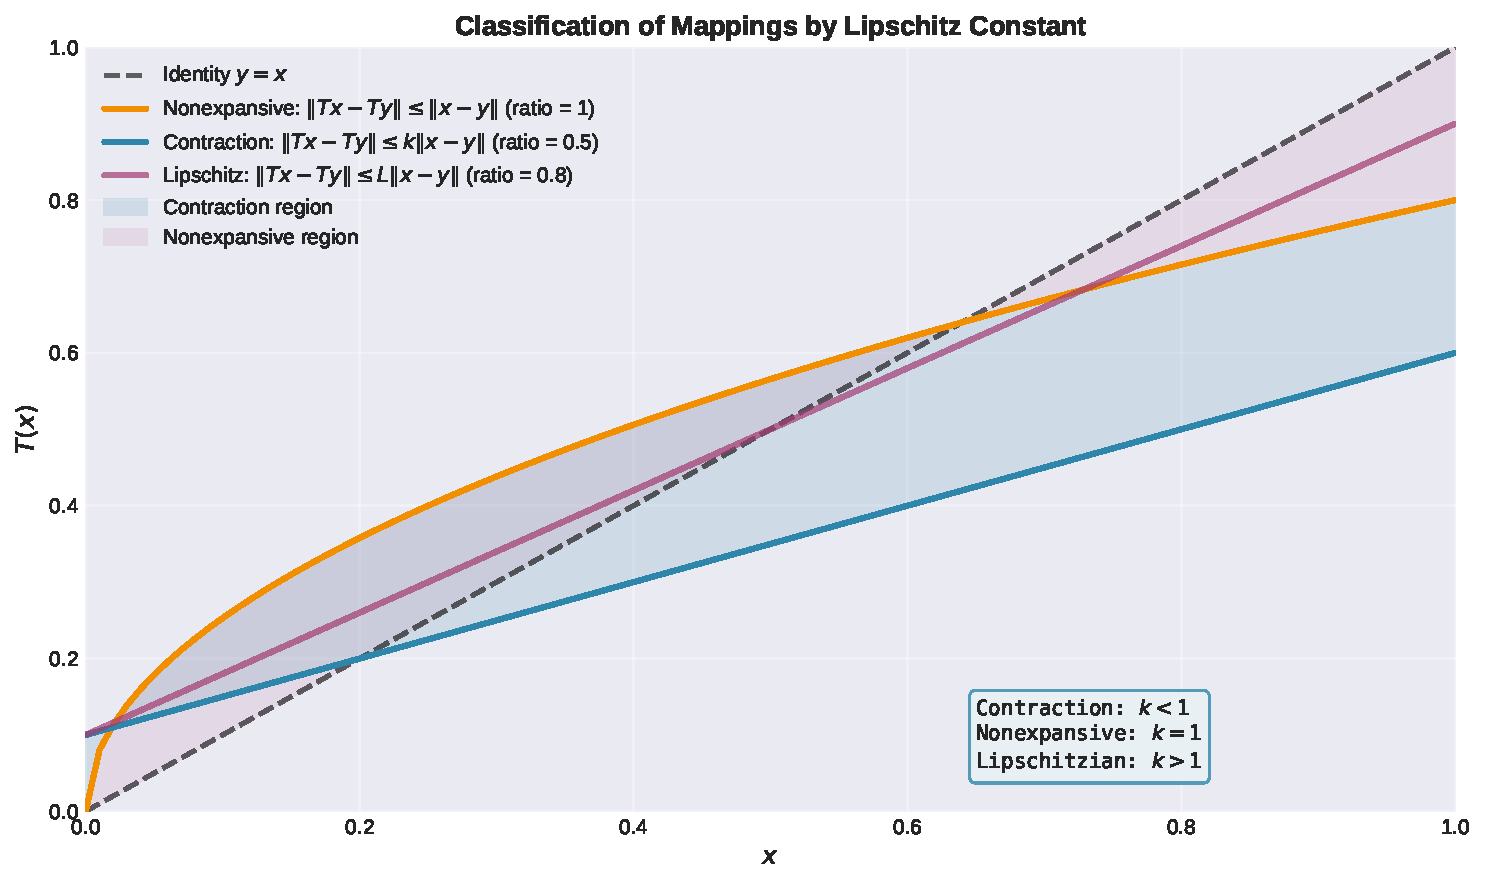
\includegraphics[width=\textwidth]{fig_lipschitz_contractive.pdf}
    \end{figure}

    \textbf{Classification by Lipschitz Constant:}
    \begin{itemize}
        \item $k < 1$: Contraction (guaranteed fixed point)
        \item $k = 1$: Nonexpansive (may have fixed points)
        \item $k > 1$: Expansive (generally no fixed points)
    \end{itemize}
\end{frame}

% Section 4: Integration with Operator Theory
\section{Integration with Banach Algebra Theory}

\begin{frame}[allowframebreaks]{Krasnoselski and Burton in Detail}
    \begin{figure}[h]
        \centering
        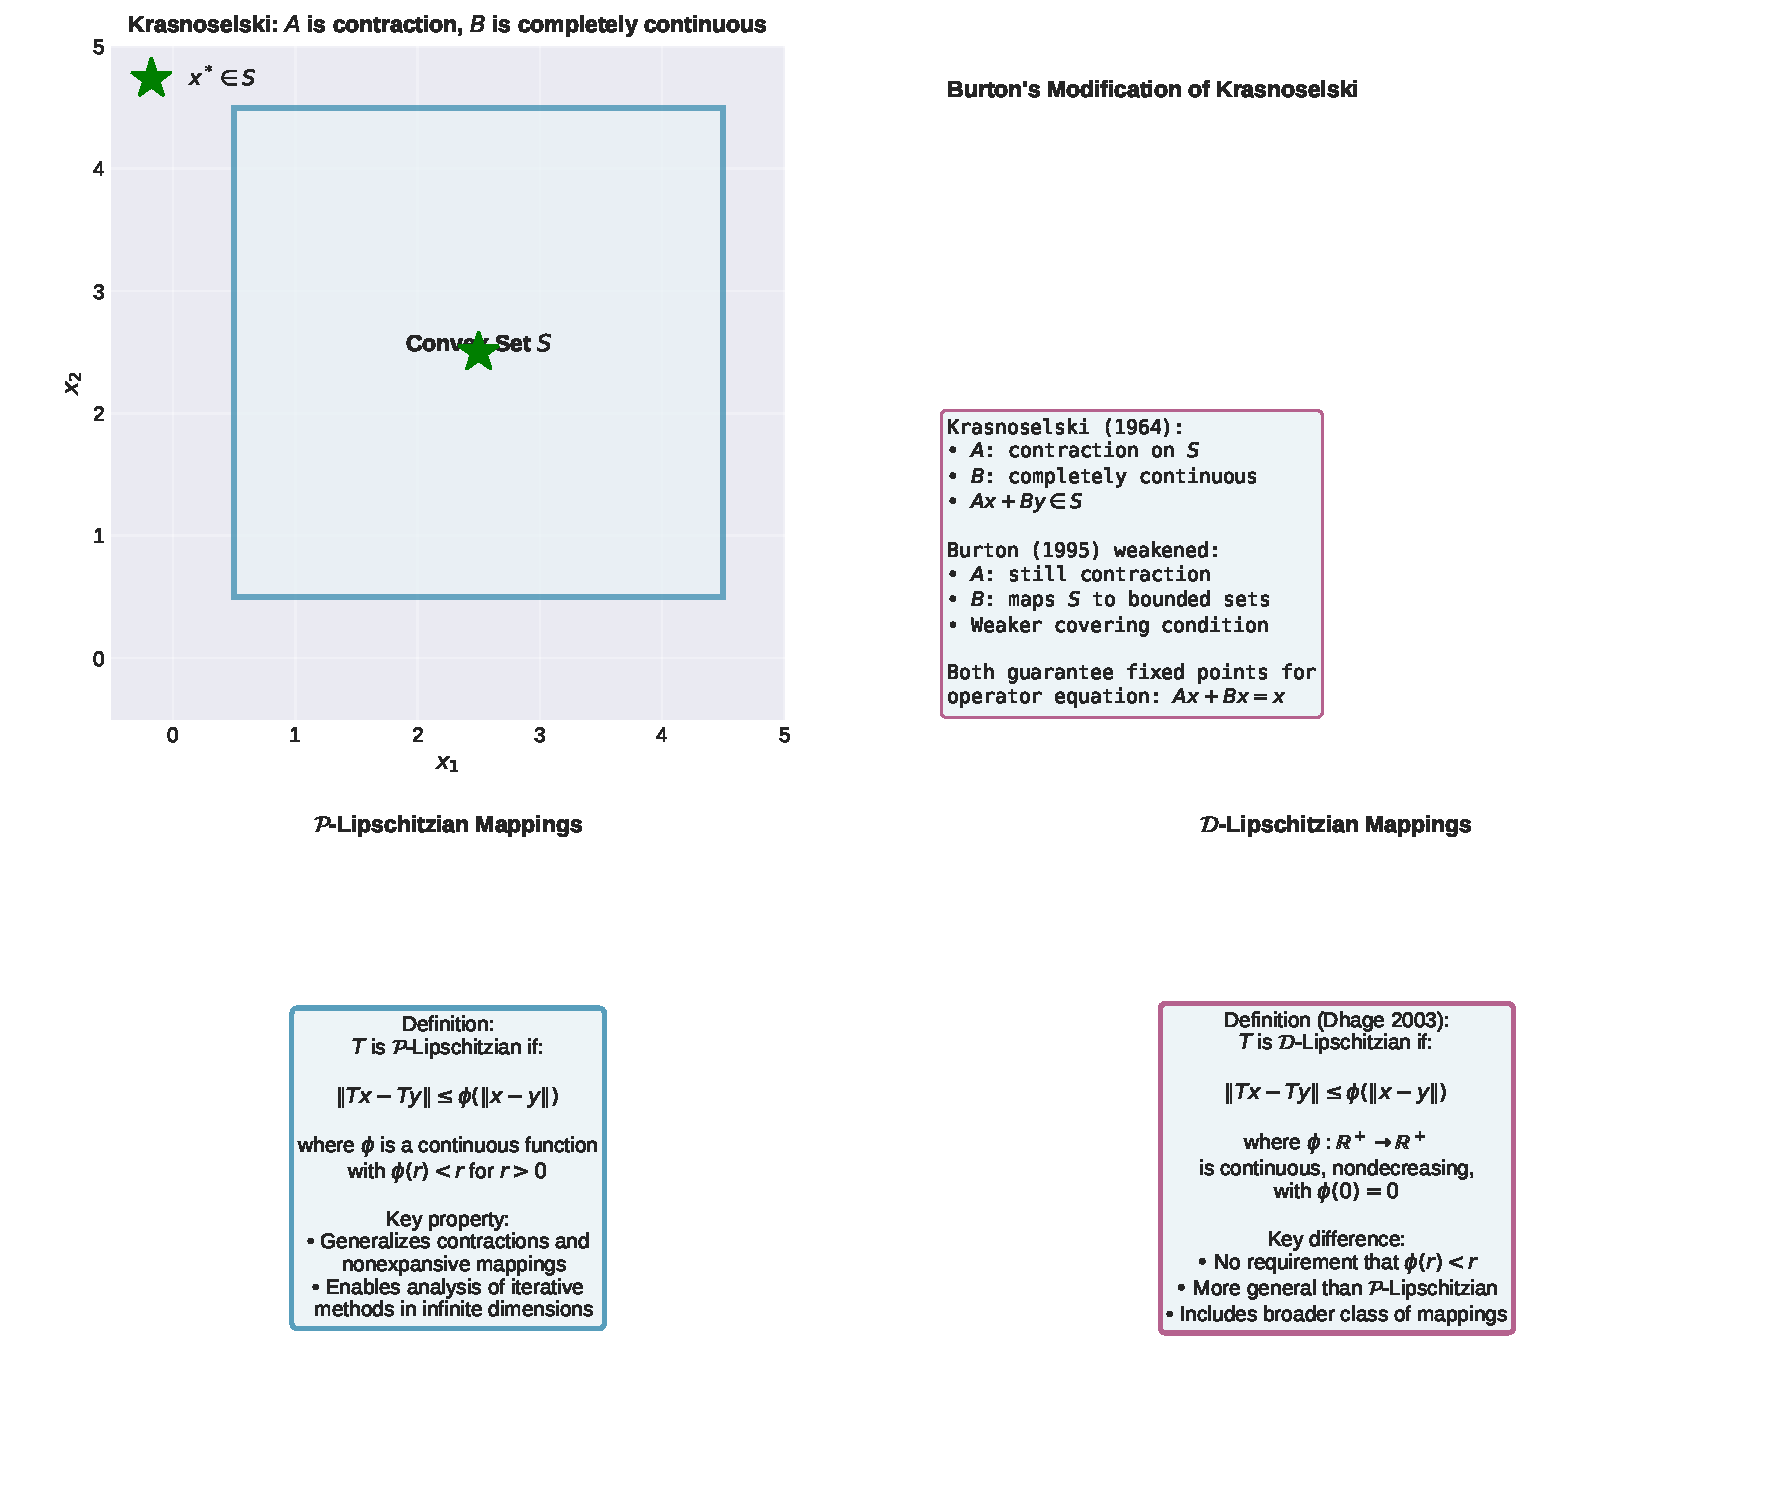
\includegraphics[width=\textwidth]{fig_krasnoselski_burton.pdf}
    \end{figure}

    \framebreak

    \textbf{Why Decompose into $A + B$?}
    \begin{enumerate}
        \item $A$ (contraction): Handles dissipative effects
        \begin{itemize}
            \item Shrinks distances: iterations converge
            \item Can handle nonlinear feedback
        \end{itemize}
        \vspace{0.2cm}
        \item $B$ (compact): Captures perturbations
        \begin{itemize}
            \item Can be unbounded but compact
            \item Allows for resonance and bifurcation effects
        \end{itemize}
    \end{enumerate}

    \vspace{0.3cm}
    \textbf{Applications:}
    \begin{itemize}
        \item Hammerstein integral equations
        \item Nonlinear Fredholm equations
        \item Semilinear PDEs with compact embeddings
    \end{itemize}
\end{frame}

\begin{frame}[fragile]{Hammerstein Integral Equations}
    \begin{problem}[Hammerstein Equation]
        Solve the nonlinear integral equation:
        \[
            x(t) = f(t) + \int_0^1 K(t,s) g(s, x(s)) \, ds, \quad t \in [0,1]
        \]
        where:
        \begin{itemize}
            \item $K(t,s)$ is the integral kernel
            \item $g$ is a nonlinear function
            \item $f$ is a given input
        \end{itemize}
    \end{problem}

    \begin{lstlisting}[language=Python, caption=Numerical solution of Hammerstein equation]
import numpy as np
from scipy.integrate import quad

# Discretized Hammerstein equation
def hammerstein_operator(x, kernel, g, f, t_points):
    """
    Compute Ax + Bg(x) where:
    A: linear part, B: nonlinear kernel integration
    """
    result = np.zeros_like(x)
    for i, t in enumerate(t_points):
        # Linear part: A*x
        result[i] = f[i]
        # Nonlinear part: integral of K(t,s)*g(s,x(s))
        def integrand(s):
            s_idx = int(s * (len(x) - 1))
            return kernel(t, s) * g(s, x[s_idx])
        integral, _ = quad(integrand, 0, 1)
        result[i] += integral
    return result

# Example: g(s, x) = x^2 (quadratic nonlinearity)
def g(s, x):
    return x**2

def kernel(t, s):
    return np.exp(-abs(t - s))

f = np.ones(10)
t_points = np.linspace(0, 1, 10)
    \end{lstlisting}
\end{frame}

\begin{frame}{Summary of Key Results}
    \begin{table}[h]
        \centering
        \small
        \begin{tabular}{|l|c|c|c|}
            \hline
            \textbf{Theorem} & \textbf{Equation} & \textbf{Conditions} & \textbf{Conclusion} \\
            \hline
            Krasnoselski & $Ax + Bx = x$ & $A$ contraction & \\
            (5.176) & & $B$ compact & Fixed point exists \\
            \hline
            Burton & $Ax + Bx = x$ & $A$ contraction & \\
            (5.177) & & $B$ bounded & Weaker conditions \\
            \hline
            $\mathcal{P}$-Lipschitz & $Ax + Bx = x$ & $A$ & \\
            (5.184) & & $\mathcal{P}$-Lipschitzian & Fixed point exists \\
            & & $B$ compact & if $M\phi(r) < r$ \\
            \hline
            $\mathcal{D}$-Lipschitz & $Ax By = x$ & $A$ & \\
            (5.185) & & $\mathcal{D}$-Lipschitzian & Fixed point exists \\
            & & $B$ compact & if $M\phi(r) < r$ \\
            \hline
            Knaster-Tarski & $f(x) = x$ & $f$ monotone & Fixed point set \\
            (5.9) & & complete lattice & is a lattice \\
            \hline
        \end{tabular}
    \end{table}
\end{frame}

% Section 5: Applications and Extensions
\section{Applications and Computational Methods}

\begin{frame}{Practical Applications}
    \textbf{In Fixed Point Theory:}
    \begin{itemize}
        \item Finding equilibrium points in dynamical systems
        \item Solving nonlinear equations with operator decomposition
        \item Existence of solutions to integral and differential equations
    \end{itemize}

    \vspace{0.3cm}
    \textbf{In Numerical Analysis:}
    \begin{itemize}
        \item Fixed point iteration methods (Newton's method variants)
        \item Successive approximation schemes
        \item Convergence analysis of iterative algorithms
    \end{itemize}

    \vspace{0.3cm}
    \textbf{In Optimization:}
    \begin{itemize}
        \item Proximal point algorithms
        \item Gradient descent and variants
        \item Splitting methods for composite problems
    \end{itemize}

    \vspace{0.3cm}
    \textbf{In Game Theory and Economics:}
    \begin{itemize}
        \item Existence of Nash equilibria
        \item Fixed points in best-response dynamics
        \item Equilibrium in market models
    \end{itemize}
\end{frame}

\begin{frame}[fragile]{Computational Implementation}
    \begin{lstlisting}[language=Python, caption=Generic fixed point iterator with monitoring]
import numpy as np
from numpy.linalg import norm

class FixedPointIterator:
    """Generic fixed point iteration method"""

    def __init__(self, operator, tol=1e-10, max_iter=1000):
        self.operator = operator
        self.tol = tol
        self.max_iter = max_iter
        self.history = []

    def iterate(self, x0):
        """Run fixed point iteration"""
        x = x0.copy()
        for n in range(self.max_iter):
            x_old = x.copy()
            x = self.operator(x)
            error = norm(x - x_old)
            self.history.append(error)

            if error < self.tol:
                print(f"Converged in {n} iterations")
                return x, self.history

            if n % 100 == 0:
                print(f"Iter {n:4d}: error = {error:.2e}")

        print("Max iterations reached!")
        return x, self.history

# Example: Banach contraction T(x) = 0.5*x + 0.1
iterator = FixedPointIterator(lambda x: 0.5*x + 0.1)
x0 = np.array([1.0, 2.0, 3.0])
solution, errors = iterator.iterate(x0)
    \end{lstlisting}
\end{frame}

\begin{frame}[fragile]{Convergence Verification}
    \begin{lstlisting}[language=Python, caption=Verifying theoretical convergence rates]
import numpy as np
import matplotlib.pyplot as plt

# Simulate convergence for different methods
def simulate_convergence(contraction_ratio, n_iter=30):
    """Simulate fixed point iteration convergence"""
    errors = np.zeros(n_iter)
    errors[0] = 1.0  # Initial error
    for n in range(1, n_iter):
        errors[n] = contraction_ratio * errors[n-1]
    return errors

# Compare different contraction ratios
fig, (ax1, ax2) = plt.subplots(1, 2, figsize=(12, 4))

# Linear scale
for k in [0.3, 0.5, 0.7, 0.9]:
    errors = simulate_convergence(k)
    ax1.plot(errors, 'o-', label=f'$k={k}$', markersize=4)
ax1.set_xlabel('Iteration $n$')
ax1.set_ylabel('Error $e_n$')
ax1.set_title('Linear Scale')
ax1.legend()
ax1.grid(True, alpha=0.3)

# Log scale
for k in [0.3, 0.5, 0.7, 0.9]:
    errors = simulate_convergence(k)
    ax2.semilogy(errors, 'o-', label=f'$k={k}$', markersize=4)
ax2.set_xlabel('Iteration $n$')
ax2.set_ylabel('Error $e_n$ (log scale)')
ax2.set_title('Log Scale')
ax2.legend()
ax2.grid(True, alpha=0.3, which='both')

plt.tight_layout()
plt.savefig('convergence_comparison.pdf')
    \end{lstlisting}
\end{frame}

% Section 6: Summary and Extensions
\section{Summary and Extensions}

\begin{frame}[allowframebreaks]{Key Theorems Summary}
    \textbf{Section 5.8: Fixed Point Theorems in Banach Algebra}
    \begin{enumerate}
        \item \textbf{Krasnoselski (1964):} Decompose $T = A + B$ where $A$ is contraction, $B$ is compact
        \item \textbf{Burton (1995):} Weaker hypothesis replacing complete continuity
        \item \textbf{$\mathcal{P}$-Lipschitzian (5.184):} Generalized contractions with function $\phi$
        \item \textbf{$\mathcal{D}$-Lipschitzian (5.185):} Further generalization (Dhage 2003)
    \end{enumerate}

    \framebreak

    \textbf{Section 5.9: Lattice-Theoretic Fixed Point Theorems}
    \begin{enumerate}
        \item \textbf{Knaster-Tarski (1927):} Monotone functions on complete lattices have fixed points
        \item \textbf{Fixed Point Lattice:} Set of fixed points forms a complete lattice
        \item \textbf{Cascading Nonexpansive Maps:} Compositions preserve fixed points in reflexive spaces
        \item \textbf{Reflexivity:} Key property ensuring weak compactness in infinite dimensions
    \end{enumerate}

    \framebreak

    \textbf{Unifying Concepts:}
    \begin{itemize}
        \item \textbf{Contractiveness:} Core property enabling guaranteed convergence
        \item \textbf{Compactness:} Enables treating perturbations
        \item \textbf{Monotonicity:} Sufficient for lattice fixed points without continuity
        \item \textbf{Decomposition:} Breaking complex problems into simpler components
    \end{itemize}
\end{frame}

\begin{frame}{Extensions and Further Reading}
    \textbf{Advanced Topics:}
    \begin{itemize}
        \item Multivalued mappings and fixed points
        \item Fixed points in metric spaces and ultrametric spaces
        \item Approximate fixed points and $\varepsilon$-fixed points
        \item Fixed point theorems in partial metric spaces
    \end{itemize}

    \vspace{0.3cm}
    \textbf{Computational Aspects:}
    \begin{itemize}
        \item Iterative schemes: Mann, Ishikawa, Krasnoselski iterations
        \item Convergence rates and acceleration techniques
        \item Parallel and distributed fixed point algorithms
    \end{itemize}

    \vspace{0.3cm}
    \textbf{Applications:}
    \begin{itemize}
        \item Differential equations: Picard-Lindelöf theorem, periodic solutions
        \item Integral equations: Hammerstein, Fredholm, Volterra equations
        \item Variational inequalities and complementarity problems
        \item Machine learning: Neural network fixed points, equilibrium models
    \end{itemize}
\end{frame}

\begin{frame}{Conclusion}
    \textbf{Main Takeaways:}
    \begin{enumerate}
        \item \textbf{Decomposition:} Complex problems can be split into manageable parts
        \begin{itemize}
            \item Contraction + compact perturbation (Krasnoselski-Burton)
            \item Monotone increasing functions on lattices (Knaster-Tarski)
        \end{itemize}
        \vspace{0.2cm}

        \item \textbf{Generalization:} From strict contractions to Lipschitzian and $\mathcal{D}$-Lipschitzian mappings
        \vspace{0.2cm}

        \item \textbf{Abstraction:} Lattice structures provide algebraic framework without topology
        \vspace{0.2cm}

        \item \textbf{Computability:} Iterations provide constructive proofs and practical algorithms
    \end{enumerate}

    \vspace{0.5cm}
    \textbf{Next Steps:}
    \begin{itemize}
        \item Apply to specific problem domains (differential equations, optimization)
        \item Study convergence rates and complexity
        \item Explore parallel and distributed implementations
    \end{itemize}
\end{frame}

\end{document}
